
\section*{Введение}

Ежегодно в России происходит рост численности населения по данным Росстата и по оценке уже к 2036~году численность составит 153,2~млн человек. Каждый человек с самого рождения стремится к удовлетворению своих амбиций, к хорошей стабильной жизни. И так уж сложилось, что  признаком успешности человека в жизни является наличие большого количества денег, сбережений, недвижимости, и, в частности, автомобилей. Для кого-то это просто средство передвижения, для кого-то показатель статуса.

Актуальность темы исследования. Одной из острых экологических проблем настоящего времени является загрязнение атмосферного воздуха. В больших городах к числу основных источников загрязнения атмосферного воздуха относится автотранспорт. Отходящие газы двигателей содержат сложную смесь из более двухсот компонентов, среди которых немало канцерогенов. Вредные вещества поступают в воздух практически в зоне дыхания человека. Поэтому автомобильный транспорт следует отнести к наиболее опасным источникам загрязнения. В настоящее время мировой автомобильный парк превысил 600~млн. единиц, из которых 83-85~\% приходится на легковые автомобили. По прогнозам, к 2030~году он достигнет 1,5~млрд. единиц.

Мировой ежегодный выброс вредных веществ от автомобилей составляет 50~млн.т. углеводородов, 200~млн.т, оксида углерода и 20~млн.т. оксидов азота. Во многих городах мира концентрации вредных веществ в воздухе, создаваемые выбросами автотранспорта, превышают стандарты качества атмосферного воздуха.

Во многих городах России выбросы автотранспорта преобладают над выбросами от стационарных источников, и уровень загрязнения воздуха превышает нормативы предельно допустимых концентраций. В связи с этим проблема снижения негативного воздействия автотранспорта на здоровье людей, воздушный и водный бассейны, растительный и животный мир, почвы весьма актуальна.

Защита атмосферы от вредных воздействий, возникающих в результате эксплуатации автомобильного транспорта, является крайне актуальной, поскольку от качества атмосферного воздуха в наибольшей степени зависит не только здоровье человека, но и в целом качество жизни на планете. Это составляет практическую значимость работы.

Цель работы: оценка влияния автотранспорта на состояние окружающей среды путем измерения и сравнения уровня загрязнения СО на разных остановочных пунктах г.~Воронежа.

Задачи исследования:
\begin{itemize}
\item оценка влияния автотранспорта на окружающую среду;
\item определение величины выбросов загрязняющих веществ от автотранспортных средств;
\item исследование загруженности автотранспортом с учетом видов автомобилей на остановочных пунктах: ''Спартак'', ''Карла Маркса'' и ''ТЮЗ'' г. Воронежа.
\end{itemize}

Объектом исследования является приземный слой атмосферы на остановочных пунктах: ''ул. Карла Маркса'', ''Кинотеатр ''Спартак'' и ''ТЮЗ'' г. Воронежа. Целью исследования – влияние выбросов от автотранспорта на состояние приземного слоя атмосферы на этих остановочных пунктах.

Всех тех, кто покупает автомобиль сейчас, однозначно должна беспокоить проблема загрязнения окружающей среды выхлопными газами автомобилей на двигателях внутреннего сгорания. Безусловно, сейчас появляется все больше средств передвижения на электрической тяге, но они гораздо дороже, и имеют свои отрицательные стороны. Человечеству нужна дешевая альтернатива бензиновым автомобилям в ближайшем будущем.

Сроки проведения работы ноябрь 2022~года.







\section{Теоретическая часть}

\subsection{Автотранспорт и его влияние на экологию города}

Автомобильный парк, являющийся одним из основных источников загрязнения окружающей среды, сосредоточен, в основном, в городах. Если в среднем в мире на 1~км$^2$ территории приходится пять автомобилей, то плотность их в крупнейших городах развитых стран в 200-300~раз выше. В настоящее время в мире насчитывается 940~млн. легковых, 80~млн. грузовых автомобилей и примерно 1,5~млн. городских автобусов.

Автомобили сжигают огромное количество ценных нефтепродуктов, нанося одновременно ощутимый вред окружающей среде, главным образом атмосфере. Поскольку основная масса автомобилей сконцентрирована в крупных и крупнейших городах, воздух этих городов не только обедняется кислородом, но и загрязняется вредными компонентами отработавших газов. Противоречия, из которых ''соткан'' автомобиль, пожалуй, ни в чём не выявляются так резко, как в деле защиты природы. С одной стороны, он облегчил человеку жизнь, с другой – отравляет её в самом прямом смысле слова. Специалисты установили, что один легковой автомобиль ежегодно поглощает из атмосферы в среднем более 4~тонн кислорода, выбрасывая с отработавшими газами примерно 800~кг окиси углерода, около 40~кг окислов азота и почти 200~кг различных углеводородов. Если помножить эти цифры на 600~млн. единиц мирового парка автомобилей, можно представить себе степень угрозы, таящейся в чрезмерной автомобилизации.
Для снижения вредного влияния автомобильного транспорта требуется вынос из городской черты грузовых транзитных потоков. Требование это зафиксировано в действующих строительных нормах и правилах, но практически соблюдается редко.

Для снижения вредного влияния автомобильного транспорта требуется вынос из городской черты грузовых транзитных потоков. Требование это зафиксировано в действующих строительных нормах и правилах, но практически соблюдается редко.

''Город без автомобиля'' мыслится как сочетание широких транспортных магистралей, где предоставляется простор для автомобильного движения, с микрорайонами, куда въезд транспорта запрещён или предельно ограничен и где люди ходят только пешком.

Эффективным мероприятием по снижению вредного влияния автомобильного транспорта на горожан является организация пешеходных зон с полным запретом въезда транспортных средств на жилые улицы. Развитие общественного транспорта в городах обуславливает необходимость поиска путей оптимального использования городских территорий, так как для перевозки одного пассажира в трамвае требуется 0,9~м$^2$, автобусе – 1,1~м$^2$, легковом автомобиле – свыше 20~м$^2$ городской территории \cite{golubev}.

''Автомобиль не роскошь, а средство передвижения'' – эти слова из известного произведения Ильфа и Петрова, звучавшие иронически, обрели в наше время реальный смысл. Более 10~млн. людей имеют автомобиль в личном пользовании. Взлёт использования личного автотранспорта произошёл в последние 15~лет.





\subsection{Классификация автомобилей}

Автомобильная промышленность в зависимости от назначения и приспособленности к дорожным условиям выпускает автомобили различных типов. По назначению автомобили делятся на пассажирские, грузовые и специальные. К пассажирским автомобилям, предназначенным для перевозки людей, относятся легковые автомобили и автобусы. Грузовые автомобили служат для перевозки различных грузов. 

Пассажирские автомобили, вмещающие не более 8~человек, называют легковыми, а вмещающие более 8~человек – автобусами.

Автобусы, предназначенные для внутри городского и пригородного общественного транспорта, называют городскими, а предназначенные для междугородних перевозок - междугородными. Число мест в автобусах в зависимости от назначения составляет 10–80.
По длине автобусы разделены на следующие классы:
\begin{itemize}
\item особо малый до 5~м;
\item малый 6–7,5~м;
\item средний 8–9,5~м;
\item большой 10,5–12~м.
\end{itemize}

Грузовые автомобили делят по грузоподъемности, т. е. по массе груза (т), который можно перевести в кузове. По грузоподъемности они делятся на классы:
\begin{itemize}
\item особо малый 0,3–1~т;
\item малый 1–3~т;
\item средний 3–5~т;
\item большой 5–8~т;
\item особо большой 8~т и более.
\end{itemize}

Автомобили специального назначения выполняют не транспортные работы. К ним относятся коммунальные автомобили для очистки и поливки улиц, пожарные, автокраны и т.д.

По приспособленности к дорожным условиям различают автомобили нормальной и повышенной проходимости. Первые имеют один, а вторые два или три ведущих моста, что позволяет им преодолевать бездорожье или плохие участки дороги.

По типу двигателя автомобили делят на имеющие карбюраторные двигатели, газовые, дизели, электродвигатели.








\subsection{Основные виды топлива, используемые в автотранспорте}

\subsubsection{Автомобильные бензины}

На автозаправках продают бензин марок \mbox{АИ-80} (он же \mbox{А-76} или \mbox{Н-80}), \mbox{АИ-92}, \mbox{АИ-95}, \mbox{АИ-98}.
Буква А означает, что бензин автомобильный, цифра - наименьшее октановое число, определенное по моторному методу; наличие буквы И указывает на то, что октановое число определено по исследовательскому методу. Автомобильные бензины, за исключением бензина \mbox{АИ-98}, разделены на летние и зимние. Зимние бензины содержат увеличенное количество легкоиспаряющихся фракций, что улучшает условие пуска двигателя.

В автомобильные бензины \mbox{А-76}, \mbox{АИ-92}, \mbox{АИ-98} добавляют антидетонатор~- тетраэтилсвинец (ТЭС) для повышения их антидетонационной стойкости. Вредные эффекты, вызываемые тетраэтилсвинцом, стали известны общественности начиная с конца 1940-х — начала 1950-х годов.

Тетраэтилсвинец — летучая жидкость при вдыхании воздуха проникает в организм через органы дыхания. Тетраэтилсвинец также может проникать в организм через неповрежденную кожу. Это вещество является сильным ядом, который избирательно поражает нервную систему, вызывая острые, подострые и хронические отравления. Хронические отравления обусловлены кумулятивным физиологическим эффектом, свойственным этому токсическому веществу. Поражается прежде всего кора головного мозга.


\begin{figure}[H]%
  \centering
  \includegraphics[width=0.4\textwidth]{src/tetraetilPb.png}
  \caption{Молекула тетраэтилсвинца} \label{p:k_marks}
\end{figure}% scale = 0.3, width=\textwidth


Для отличия обыкновенного бензина от этилированных, последние окрашивают в зеленый (\mbox{А-76}), синий (\mbox{АИ-92}) и желтый (\mbox{АИ-98}) цвета.




\subsubsection{Дизельное топливо}

Топливо, применяемое для автомобильных дизельных двигателей, представляет собой тяжелые нефтяные фракции. Оно должно обеспечивать мягкую и плавную работу двигателей, отвечать условиям надежной подачи его в цилиндры топливоподающей аппаратурой, не оставлять значительного нагара, быть свободным от механических примесей и воды, содержать наименьшее количество органических кислот и серы. Дизельное топливо должно иметь определенную вязкость и возможно более низкую температуру застывания и воспламенения.

В настоящее время по \mbox{ГОСТ 305-82}, \mbox{ГОСТ 1667-68} выпускаются сорта дизельного топлива: Л - летнее, З - зимнее, А - арктическое. Каждое из названных топлив делится на две подгруппы: первая с содержанием серы не более 0,2~\% и вторая содержание не превышает 0,5~\%.

Летнее дизельное топливо ДЛ можно применять только при температуре окружающего воздуха выше 0~°С. Когда температура опускается до минус 20~°С, следует применять зимнее топливо З, а при морозах, достигающих -30~°С топливо ДЗ, при более низких температурах применяют арктическое топливо. Однако применять арктическое топливо при температуре выше минус -30~°С нельзя.



\subsubsection{Топливо для газобаллонных автомобилей}

Горючие газы, используемые в газобаллонных автомобилях, могут быть естественными и искусственными. Естественные газы добывают из подземных газовых или нефтяных скважин. Искусственные газы являются побочными продуктами, получаемыми на химических или металлургических заводах. 

Установлены следующие марки газов:
\begin{itemize}
\item СПБТЗ - смесь пропана и бутана техническое зимнее;
\item СПБТЛ - смесь пропана и бутана техническое летнее;
\item БТ - бутан технический.
\end{itemize}

Сжиженный пропан - бутановый газ согласно стандарту должен содержать пропана зимой не менее 90~\%, а летом не менее 70~\%. Газ не должен содержать механических примесей, воды, водорасстворимых кислот, щелочей и других загрязняющих веществ.

Сжатыми называют газы, которые при обычной температуре окружающей среды и высоком давлении до 20~тыс.~кН/м$^2$ сохраняют газообразное состояние.
Сжиженными газами называют такие, которые переходят из газообразного состояния в жидкое при нормальной температуре и небольшом давлении до 1600~кН/м$^2$.
Для газобаллонных автомобилей использование сжиженных газов предпочтительнее, чем сжатых 
\cite{mihailovsky}.










\newpage
\subsection{Причины дымления автомобилей}

Причины дымления автомобилей различны: неисправность двигателя, неотлаженность системы питания или зажигания. Если все автомобильные двигатели будут правильно отрегулированы, то выброс вредных веществ в атмосферу уменьшится в 3-5~раз. Экономия денег на техобслуживании приводят к тому, что автомобили неделями, а то и месяцами развозят по улицам ядовитый газ. Плохо накачанные шины не только быстрее изнашиваются, но и увеличивают сопротивление движению, а значит, больше сжигается горючего. Сильно сказывается на окружающей среде сотяние автомобилей в ''пробках'' со включенными двигателями.

Неумелое поведения водителя за рулём (неправильный выбор скоростей движения, резкие разгоны и торможения, превышение установленной скорости), а так же самостоятельная регулировка (увеличение частоты вращения на холостом ходу) и нарушение инструкций по эксплуатации автомобиля, нередко приводит к увеличению загрязнения окружающей среды. Поэтому разъяснительная работа среды водителей автомобилей в этом направлении очень важна.









\subsection{Краткая характеристика монооксида углерода СО (угарного газа) и его влияние на природную среду и человека}

Образуется в результате неполного сгорания углерода в моторном топливе. Ядовитый газ без цвета и запаха. 

\begin{figure}[H]%
  \centering
  \begin{minipage}[h]{0.4\linewidth}
    \center{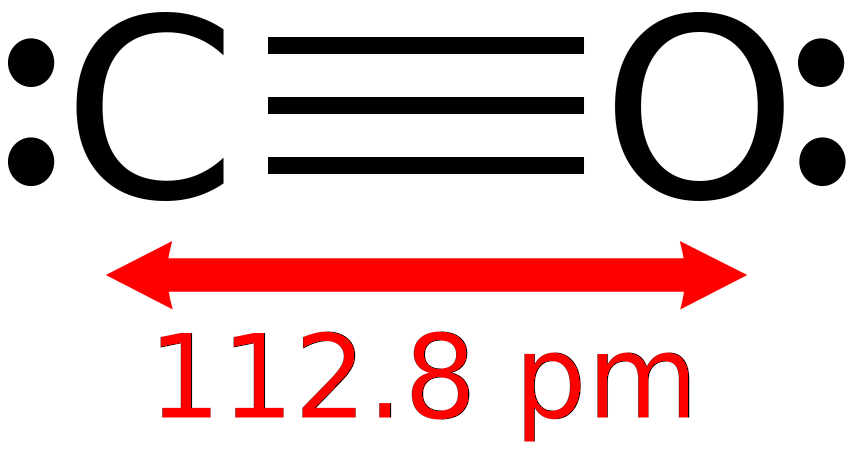
\includegraphics[width=0.8\textwidth]{src/Carbon_monoxide_2D.png}}
  \end{minipage}
  \hfill
  \begin{minipage}[h]{0.4\linewidth}
    \center{\includegraphics[width=0.8\textwidth]{src/Carbon-monoxide-3D-vdW.png}}
  \end{minipage}
  \caption{Молекула монооксида углерода СО} \label{p:Carbon_monoxide}
\end{figure}% scale = 0.3, width=\textwidth

При вдыхании связывается с гемоглобином крови, вытесняя из нее кислород, в результате чего наступает кислородное голодание, сказывающееся прежде всего на центральной нервной системе. Среднесуточная предельно допустимая концентрация (ПДК) по монооксиду углерода составляет \directlua{rnd2(t.PDK)}~мг/м$^3$.

Высокая концентрация монооксида углерода даже при кратковременном воздействии может привести к смерти: небольшие дозы вызывают головокружение, головную боль, чувство усталости и замедление реакции у водителя. Повышение концентрации монооксида углерода часто возникает в туннелях (до 70~ПДК), в потоке транспортных средств при интенсивном движении (до 60~ПДК), в гаражах. Известны случаи трагической гибели людей, запускающих двигатели автомобилей при закрытых воротах гаража. В одноместном гараже смертельная концентрация СО возникает уже через 2-3~мин. после включения стартера. В холодное время года, остановившись для ночлега, водители иногда включают двигатель для обогрева салона. Из-за проникновения монооксида углерода в кабину такой ночлег может оказаться последним.

Воздействие атмосферных загрязнений на здоровье можно подразделить на два вида в зависимости от времени проявления эффекта: острое, сказывающееся в период или непосредственно вслед за повышением концентрации токсичного вещества, и хроническое воздействие, результат которого проявляется не сразу, а через некоторое время, иногда через годы. Как в первом, так и во втором случаях атмосферные загрязнения могут быть непосредственной причиной развития заболевания или оказывать не специфическое отягощающее воздействие.

Проникновение угарного газа повышенной концентрации через органы дыхания в наши дни привело к существенному изменению состояния организма. Развилась патологическая повышенная чувствительность организма. Ощутимыми темпами происходит накопление наследственных пороков. Широкое распространение получили хронический бронхит, а также прежде формы легочной патологии, такие как аллергические воспаления альвеол. Увеличилось число больных бронхиальной астмой, относящейся к наиболее тяжелым проявлениям аллергии. Особую тревогу вызывает увеличение количества больных раком легкого, который по своей распространительности у мужчин вышел на первое место среди онкологических заболеваний. Потому как остро стоит проблема защиты воздушной среды от всех видов загрязнений.




